\documentclass[12pt]{article}
\usepackage{amsmath,amsfonts,amsthm,amssymb,graphicx,authblk}
\usepackage[font={footnotesize,singlespacing},labelfont=bf]{caption}
\usepackage{blkarray, bm} 
\usepackage{float,afterpage}
\usepackage[running,mathlines]{lineno}

\usepackage[verbose,letterpaper,tmargin=2.54cm,bmargin=2.54cm,lmargin=2.54cm,rmargin=2.54cm]{geometry}
\usepackage[authoryear,sort]{natbib}
\usepackage[dvipsnames]{xcolor}
\usepackage{hyperref}

\usepackage[compact,small]{titlesec}
\usepackage[moderate]{savetrees}

\usepackage{enumitem}
\setlist{topsep=.1em,itemsep=-0.2em,leftmargin=0.75cm}

\setlength{\parindent}{0.35in}
% \usepackage[sc]{mathpazo} %Like Palatino with extensive math support
\usepackage[scale=1]{newtxtext,newtxmath} 

\usepackage{siunitx}

\usepackage[nodisplayskipstretch]{setspace} 

% Coloring of R code listings
\usepackage[formats]{listings}
\usepackage{color}
\definecolor{mygreen}{rgb}{0.1,0.5,0.1}
\definecolor{mygray}{rgb}{0.5,0.5,0.5}
\definecolor{mymauve}{rgb}{0.58,0,0.82}
\definecolor{mygrey}{rgb}{0.3,0.3,0.1}
\lstset{
	language=R,
	otherkeywords={data.frame},
	basicstyle=\normalsize\ttfamily, 
	commentstyle=\normalsize\ttfamily,
	keywordstyle=\normalsize\ttfamily,
	stringstyle=\color{mymauve}, 
	commentstyle=\color{mygreen},
	keywordstyle=\color{blue},
	showstringspaces=false, xleftmargin=2.5ex,
	columns=flexible,
	literate={~}{{$\sim \; \; $}}1,
	alsodigit={\.,\_},
	deletekeywords={on,by,data,R,Q,mean,var,sd,log,family,na,options,q,weights,effects,matrix,nrow,ncol,wt,fix,distance},
}
\lstset{escapeinside={(*}{*)}} 

\lstdefineformat{Rpretty}{
	; = \space,
	\, = [\ \,\]]\string\space,
	<- = [\ ]\space\string\space,
	\= = [\ ]\space\string\space}


%\usepackage{lineno}
\renewcommand{\refname}{Literature Cited}
\renewcommand{\floatpagefraction}{0.9}
\renewcommand{\topfraction}{0.99}
\renewcommand{\textfraction}{0.05}

\clubpenalty = 10000
\widowpenalty = 10000

\sloppy 

\usepackage{ifpdf}
\ifpdf
\DeclareGraphicsExtensions{.pdf,.png,.jpg}
\usepackage{epstopdf}
\else
\DeclareGraphicsExtensions{.eps}
\fi

% commands for commenting
\newcommand{\tom}[2]{{\color{red}{#1}}\footnote{\textit{\color{red}{#2}}}}
\newcommand{\steve}[2]{{\color{blue}{#1}}\footnote{\textit{\color{blue}{#2}}}}
\newcommand{\revise}[1]{{\color{Mahogany}{#1}}}
%%%%%%%%%%%%%%%%%%%%%%%%%%%%%%%%%%%%%%%%%%%%% 
%%% Just for commenting
%%%%%%%%%%%%%%%%%%%%%%%%%%%%%%%%%%%%%%%%%%%%
\usepackage[dvipsnames]{xcolor}
\newcommand{\comment}{\textcolor{blue}}
\newcommand{\new}{\textcolor{red}}

\newcommand{\be}{\begin{equation}}
	\newcommand{\ee}{\end{equation}}

\newcommand{\red}{\textcolor{red}}

\sloppy

\begin{document}


% ######################## Appendices ##############################
\newpage 
\clearpage 
\appendix

\renewcommand{\thetable}{S-\arabic{table}}
\renewcommand{\thefigure}{S-\arabic{figure}}
\renewcommand{\thesection}{S.\arabic{section}}
\renewcommand{\theequation}{S\arabic{equation}}

\setcounter{page}{1}
\setcounter{equation}{0}
\setcounter{figure}{0}
\setcounter{section}{0}
\setcounter{table}{0}

\begin{spacing}{1.35} 
	\linenumbers
	\centerline{\Large{\textbf{Supporting Information}}}
	
	\section{The Jones-Pewsey (2009) sinh-arcsinh distributions} 
	\label{sec:SHASHdist} 
	\citet{jones-pewsey-2009} introduced a tractable generalization of the Normal distribution with two 
	additional parameters determining asymmetry (skewness), and tail weight (kurtosis) which can be either 
	lighter or heavier than the Gaussian. The generalizatin is defined through transformation of the
	Normal distribution using the hyperbolic sine function (sinh) and its inverse (asinh), 
	as follows. The base distribution $f_{\epsilon,\delta}$  is the 
	probability density of the random variable $X_{\epsilon,\delta}$ where  
	\be
	Z = \sinh (\delta \; \mbox{asinh}(X_{\epsilon,\delta}) - \epsilon)
	\label{eqn:JP1}
	\ee
	and $Z$ has a Normal(0,1) distribution. Equivalently, 
	\be
	X_{\epsilon,\delta} = \sinh \left( \delta^{-1} \big[\mbox{asinh}(Z) + \epsilon \big] \right), \quad Z \sim \mathcal{N}(0,1).
	\label{eqn:JP2}
	\ee
	Parameters $\delta=1, \; \epsilon=0$ give the Normal(0,1) distribution. Skewness has the sign of $\epsilon$, and
	$\delta > 0$ controls tail weight, with heavier than Gaussian tails for $\delta<1$ and lighter than Gaussian tails for $\delta > 1$. We show below that the nonparametric kurtosis (eqn. \eqref{eqn:NPkurt} in the main text) depends 
	only on $\delta$, not on any of the other three parameters. 
	
	The density function for $X_{\epsilon,\delta}$ is given by \citet[][eqn. 2]{jones-pewsey-2009}, 
	\be
	\begin{aligned}
		f_{ \epsilon,\delta}(x) & = C(x) \exp\{-S(x)^2/2\} \{2\pi(1+x^2)\}^{-1/2}  \\
		\mbox{ where }  S(x) & =  \mbox{sinh}(\delta \mbox{ asinh}(x)- \epsilon), \\
		C(x)  & =  \sqrt{1 + S(x)^2} = \mbox{cosh}(\delta \mbox{ asinh}(x)- \epsilon).
	\end{aligned} 
	\ee
	The attainable combinations of skewness and kurtosis are 
	very broad compared to other families, and come very close to the theoretical limit of
	kurtosis as a function of skewness \citep[][Fig.  2]{jones-pewsey-2009}. 
	Additionally, eqn. \eqref{eqn:JP2} makes it straightforward to generate random numbers and to compute 
	the probability density, cumulative distribution, and quantile functions. 
	There are also analytic formulas for the first four non-central 
	moments \citep[][p. 764]{jones-pewsey-2009} in terms of the Bessel function $K_{\nu}$, which is
	\texttt{BesselK} in base R and \texttt{besselk} in \textsc{Matlab} and GNU \textsc{Octave}.
	
	\citet{jones-pewsey-2009} defined a four-parameter distribution with location 
	parameter $\mu$ and scale parameter $\sigma$ as the distribution of $\mu + \sigma X_{\epsilon, \delta}$, 
	which has density function 
	\be
	f_{\mu, \sigma,  \epsilon,\delta}(x)  = \sigma^{-1}f_{ \epsilon,\delta}( \sigma^{-1}(x - \mu)). 
	\label{eqn:JP4} 
	\ee
	Terminology on this distribution has become somewhat confused. In the \textbf{mgcv} R package 
	it is called \texttt{shash}, while in the \textbf{gamlss} package it is called \texttt{SHASHo2} 
	and \texttt{SHASH} is a related but different distribution. To sidestep 
	this confusion we refer to \eqref{eqn:JP4} as the JP4 distribution (``Jones-Pewsey 4 parameter''), 
	and refer to \eqref{eqn:JP2} as JP2. 
	
	As is the case for most four-parameter distribution families, 
	the location parameter $\mu$ is not the mean of the JP4 distribution, 
	and $\sigma$ is not the standard deviation (additionally, $\epsilon$ is not the skew and $\delta$ is not the kurtosis). 
	We therefore define a new four-parameter distribution family, JPS, by shifting and scaling JP2
	so that the location parameter $\mu$ is the mean, and the scale parameter $\sigma$ is the standard deviation. 
	This form can then be used in custom likelihood functions that ``import'' the fitted mean 
	and standard deviation from a Gaussian pilot model, in the same way that the skewed $t$ distribution 
	was used in our lady orchid case study. 
	
	Let $m(\epsilon,\delta)$ and $s(\epsilon, \delta)$ denote the mean and standard deviation of the 
	JP2 distribution. Then define 
	\be  
	X_{JPS} = \mu \; + \; \sigma \left(\frac{X_{\epsilon,\delta} - m(\epsilon,\delta)}{s(\epsilon,\delta)}\right).
	\ee
	The right-hand term in parentheses has mean 0 and variance 1, so 
	$X_{JPS}$ has mean $\mu$ and variance $\sigma^2$, with $\epsilon$ and $\delta$ controlling skewness
	and tail weight as in JP2. Because $\mu$ and $\sigma$ have no effect on the nonparametric kurtosis, 
	JPR retains the property that nonparametric kurtosis only depends on $\delta$, not on the other three parameters. 
	
	Omitting some algebra, $X_{JPS}$ has cumulative distribution function 
	\be
	Pr(X_{JPS} \le x)  = Pr\left(X_{\epsilon,\delta} \le  m(\epsilon,\delta) + \frac{s(\epsilon,\delta)}{\sigma}(x - \mu)\right).
	\ee
	Differentiating both sides with respect to $x$, the probability distribution function for $X_{JPS}$ is 
	\be
	f_{JPS}(x \vert \mu, \sigma, \epsilon, \delta) =  \frac{s(\epsilon,\delta)}{\sigma} 
	f_{ \epsilon,\delta}\left(m(\epsilon,\delta) + \frac{s(\epsilon,\delta)}{\sigma}(x - \mu) \right) 
	\ee
	
	Eqn. \eqref{eqn:JP2} shows that the JP2 distribution depends on $\epsilon$ only through 
	the ratio $\epsilon/\delta$, and hence the same is true for JPS. 
	We have found that this property can be problematic for parameter estimation, 
	because of the resulting ridge in the likelihood surface with constant  
	$\epsilon/\delta$. Another problem is that when $\delta$ is large, changes 
	in $\epsilon$ have little effect. 
	
	To avoid those problems, we recommend writing likelihood functions in terms of 
	skewness and kurtosis parameters $\lambda$ and $\tau$, defined by 
	$\delta = e^{-\tau}, \; \epsilon =  \delta \lambda$ in the 
	JPS distribution. We will refer to this as the JPR distribution, with probability density 
	\be
	f_{JPR}(x \vert \mu, \sigma, \lambda, \tau) = f_{JPS}(x \vert \mu, \sigma, e^{-\tau}\lambda,  e^{-\tau}). 
	\ee
	$\lambda$ can take any real value, and the distribution's skewness has the same sign as $\lambda$. 
	$\tau$ also can take any real value, with negative values giving thinner than Gaussian tails 
	and positive values giving fatter than Gaussian tails. Because $\delta$ depends only on $\tau$, 
	JPR also has the property that the nonparametric kurtosis depends only on the tail-weight parameter $\tau$. 
	
	It is still the case that the ordinary skewness and kurtosis depend on both $\lambda$ and $\tau$, but the
	``crosstalk'' is weaker than that between $\epsilon$ and $\delta$ (in particular, the tail-weight parameter
	has much less effect on the skewness).  
	As a result, we found that likelihood optimization is numerically more stable when the likelihood function is 
	written as a function of $\tau$ and $\lambda$ rather than $\delta$ and $\epsilon$. 
	
	R code for the JP2, JPS, and JPR distributions with the usual \texttt{d,p,q,r} functions are provided 
	in the script \texttt{JP\_funs.R} in our R code archive. 
	
	\emph{Proof that NP kurtosis of JP2 depends only on $\delta$}: 
	Let $Z_\alpha$ denote the $\alpha$ percentile of a standard
	Normal distribution, $X_\alpha$ the $\alpha$ percentile of $X_{\epsilon, \delta}$ and 
	$\lambda =  \epsilon/\delta$. Then from \eqref{eqn:JP2}
	we have 
	\be
	\begin{aligned}
		X_{1-\alpha} & = \mbox{sinh} \left[ \lambda  + \delta^{-1} \mbox{asinh}(Z_{1-\alpha}) \right] ,  \\
		X_{\alpha} & = \mbox{sinh} \left[ \lambda  + \delta^{-1} \mbox{asinh}(Z_{\alpha}) \right]
		= \mbox{sinh} \left[ \lambda + \delta^{-1} \mbox{asinh}(-Z_{1-\alpha}) \right] \\
		& = \mbox{sinh} \left[ \lambda - \delta^{-1} \mbox{asinh}(Z_{1-\alpha}) \right]. 
	\end{aligned}
	\ee
	Thus  
	\be
	X_{1-\alpha} - X_{\alpha} = \mbox{sinh}(\lambda + b) - \mbox{sinh}(\lambda - b)
	\ee
	where $b = \delta^{-1}\mbox{asinh}(Z_{1-\alpha})$. We can apply the subtraction formula for sinh (eqn. 4.5.42
	in \citet{abram-steg}), namely\footnote{It's also on Wikipedia, and today it's correct, but tomorrow could
		be different.}
	\be 
	\mbox{sinh } z_1 - \mbox{sinh } z_2  = 2 \mbox{cosh}\left( \frac{z_1 + z_2}{2}\right) \mbox{sinh}\left( \frac{z_1 - z_2}{2}\right), 
	\ee  
	obtaining 
	\be
	X_{1-\alpha} - X_{\alpha} =  2 \mbox{cosh}(\lambda) \mbox{sinh}(b).
	\ee  
	The value of $b$ is independent of $\epsilon$. The $\epsilon$-dependent factor $2 \mbox{cosh}(\lambda)$ 
	cancels in the numerator and denominator of the formula for nonparametric kurtosis. \scalebox{1.25}{$\square$}
	
	\section{Estimating random effects in non-Gaussian models using shrinkage}
	\label{sec:shrinkageFits}
	Specialized software for fitting mixed effects models only allow a subset, usually a small subset, of the distributions that 
	are useful for modeling growth.\footnote{The \textbf{gamlss} package includes many distributions, but in our experience even with 
		simple random effects structure the fitting algorithms often fail to converge reliably.} One way past this limitation is Bayesian estimation. Here we describe another option, 
	introduced by \citet{link-nichols-1994} and \citet{gould-nichols-1998}: 
	fitting the model in a fixed effects framework by Maximum Likelihood, followed by shrinkage of coefficient estimates. 
	None of the ideas here are original. This section overlaps Appendix S1 of \citet{metcalf-etal-2015}, the only new wrinkle
	being the application to non-Gaussian models.
	
	We explain shrinkage using a simple model fitted to some growth data 
	on the bunchgrass \emph{Pseudoroegneria spicata} from \cite{adler-weak-dryad}. 
	The fitted model includes random effects for across-year variation in the slope and 
	intercept of future size (log area) as a function of initial size. We assume that initial size 
	and year are the only covariates, and we assume that growth increments 
	follow a skew-Normal distribution with nonconstant variance and constant skew parameter. 
	Code for this example is in the script \texttt{SimpleShrinkageExample.R}. 
	
	The fitted growth model assumes that the skew and kurtosis parameters are functions
	of the location parameter; this dominated $(\Delta AIC \approx 30)$ the analogous  
	model with skew and kurtosis depending on initial size.   
	We fitted this model by MLE with all between-year variation appearing as fixed effects. 
	The appropriate design matrix can be constructed using the \texttt{model.matrix} function: 
	\begin{lstlisting}
		U = model.matrix(~year + init.size:year - 1, data=growthData)
	\end{lstlisting}
	If there are $T$ years, the matrix \texttt{U} has $2T$ columns corresponding to $T$ annual 
	intercepts and $T$ annual slopes. 
	
	Using this design matrix, we can write a log-likelihood function for use with 
	the \textbf{maxLik} package, using a log link function for the variance parameter 
	because it is necessarily positive: 
	\begin{lstlisting}
		LogLik=function(pars,new.size,U){
			pars1 = pars[1:ncol(U)]; pars2=pars[-(1:ncol(U))];
			mu = U%*%pars1;  
			sigma = exp(pars2[1]+pars2[2]*mu);
			dSN1(new.size, mu=mu, sigma=sigma, nu=pars2[3], log=TRUE)
		}
	\end{lstlisting} 
	Parameters and their standard errors can then be estimated, starting from a random guess: 
	\begin{lstlisting}
		start=c(runif(ncol(U)), rep(0,3))
		out=maxLik(logLik=LogLik,start=start, new.size=simData$new.size,U=U,
		method="BHHH",control=list(iterlim=5000,printLevel=1),finalHessian=TRUE);
		coefs = out$estimate; # parameters
		V = vcov(out); SEs = sqrt(diag(V));	# standard errors 
	\end{lstlisting}  
	In real life we would repeat the optimization several times with different starting values, 
	to be confident that optimal parameter values had been found. 
	
	Focus now on the year-specific intercept parameters $\hat{a}_t, t = 1,2,\cdots T$. 
	We can view the year-specific estimates $\hat{a}_t$ as consisting of unobserved true values $a_t$ plus sampling error:
	\be
	\hat{a}_t= a_t + \varepsilon_t 
	\ee
	Because of sampling errors, the expected sample variance of the estimates $\hat{a}_t$ is larger 
	than the true across-year variance in the parameter, which is undesirable if population projections are made
	by random sampling from the estimated year-specific parameters (analogous to ``matrix selection'' for stochastic
	matrix models). However, the approximate variance-covariance matrix $\hat{V}$ of the sampling errors, \texttt{V} in the code 
	above, can be used to correct for this upward bias.   
	
	To make the correction we assume that the estimates $\hat{a}_t$ are unbiased, that is
	\be
	\mathbb{E}(\varepsilon_t \vert a_t) = 0.    
	\ee
	We also adopt the standard mixed-model assumption that the $a_t$ are drawn 
	independently from some fixed distribution with unknown variance $\sigma^2$. 
	These are optimistic assumptions, but not excessively so. If the assumptions of maximum likelihood are satisfied, 
	the bias in parameter estimates is asympototically negligible compared to the standard error. 
	The terms resulting from non-independence can only be reliably estimated if 
	the autocorrelations fall to nearly zero within lag $m \ll T$, 
	and in that case the autocorrelation correction term is small (see eqn. (1) in \citet{gould-nichols-1998}). 
	We therefore recommend proceeding on the assumption that the $\hat{a}_t$ are independent. 
	
	Let $S^2$ denote the sample variance of the estimates $\hat{a}_t$. It can then be shown that 
	\be
	\mathbb{E}(S^2) = \sigma^2  + \frac{1}{T}\sum\limits_{t=1}^T \mathbb{E} Var(\varepsilon_t) 
	- \frac{1}{T(T-1)}\sum\limits_{i=1}^{j-1} \sum\limits_{j=1}^T \mathbb{E}Cov(\varepsilon_i, \varepsilon_j). 
	\label{eqn:biasTerms}
	\ee
	This is equivalent to eqn. (1) in \citet{gould-nichols-1998} without the term that 
	accounts for temporal autocorrelation. 
	
	The terms besides $\sigma^2$ on the right-hand of \eqref{eqn:biasTerms} makes $S^2$ a biased estimated of $\sigma^2$. 
	However, those terms correspond to entries in the variance-covariance matrix $V$, so we can use $\hat{V}$ to remove 
	the bias: 
	\be
	\hat{\sigma^2}  = S^2 - \frac{1}{T}\sum\limits_{t=1}^T \hat{V}_{t,t} + 
	\frac{1}{T(T-1)}\sum\limits_{i=1}^{j-1} \sum\limits_{j=1}^T \hat{V}_{i,j}. 
	\label{eqn:hatSigma}
	\ee
	$\hat{\sigma^2}$ is the estimated variance of the distribution from which the $a_t$ are assumed
	to be drawn. 
	
	We can similarly adjust the year-specific estimates to compensate for the expected impact of sampling error. Several methods  
	have been proposed; following \citet{metcalf-etal-2015} we recommend the method used in the 
	capture-recapture analysis software Mark \citet{cooch-white-2020}, 
	\be
	\widetilde{a}_t = \bar{\hat{a_t}} + \sqrt{\frac{\hat{\sigma}^2}{\hat{\sigma}^2 + \hat{V}_{t,t}}}\left (\hat{a_t} - \bar{\hat{a_t}} \right). 
	\label{eqn:ShrinkLess}
	\ee
	The name ``shrinkage'' comes from the fact that each estimate is adjusted towards the overall mean, with 
	larger adjustments of values with higher estimated sampling error variance, $\hat{V}_{t,t}$. 
	The expected sample variance of the adjusted estimates $\widetilde{a}_t$ is very close to $\hat{\sigma^2}$. 
	The $\widetilde{a}_t$ therefore approximate the actual amount of parameter variation, and are analogous to the 
	year-specific estimated random effects from a mixed effects model. 
	
	The take-home message is that estimating random effects from fitted year-specific regression 
	coefficients is very simple. Continuing from the last code listing above: 
	\begin{lstlisting}
		# Variance-covariance matrices for intercepts and slopes
		V1 = V[1:T,1:T]; V2 = V[(T+1):(2*T),(T+1):(2*T)]; 
		# Extract year-specific intercepts, center them to zero   
		fixed.fx = coefs[1:T]; fixed.fx = fixed.fx-mean(fixed.fx); 
		
		# Estimate sigma^2
		var.hat = mean(fixed.fx^2) - mean(diag(V1)) + 
		(sum(V1)-sum(diag(V1)))/(2*T*(T-1)); 
		
		# Shrink deviations from the mean 
		shrinkRanIntercept = fixed.fx*sqrt(var.hat/(var.hat + diag(V1)));
		
		# Do it all again for the slopes 
		fixed.fx2 = coefs[(T+1):(2*T)]; fixed.fx2 = fixed.fx2-mean(fixed.fx2); 
		var2.hat = mean(fixed.fx2^2) - mean(diag(V2)) + 
		(sum(V2)-sum(diag(V2)))/(2*T*(T-1)); 
		shrinkRanSlope = fixed.fx2*sqrt(var2.hat/(var2.hat + diag(V2))); 
	\end{lstlisting}
	
	Figure \ref{fig:compareShrinkage} shows the results for one artificial ``data'' set, having $T=22$ years and growth measurements on 
	about 175 individuals per year on average. The true random year effects (that were used to generate the data) are recovered
	with good accuracy and no bias. In particular there is no sign of extreme values being pulled in too far
	towards the mean, which would cause an S-shaped graph of estimated versus true values. 
	
	\begin{figure}[tbp]
		\centerline{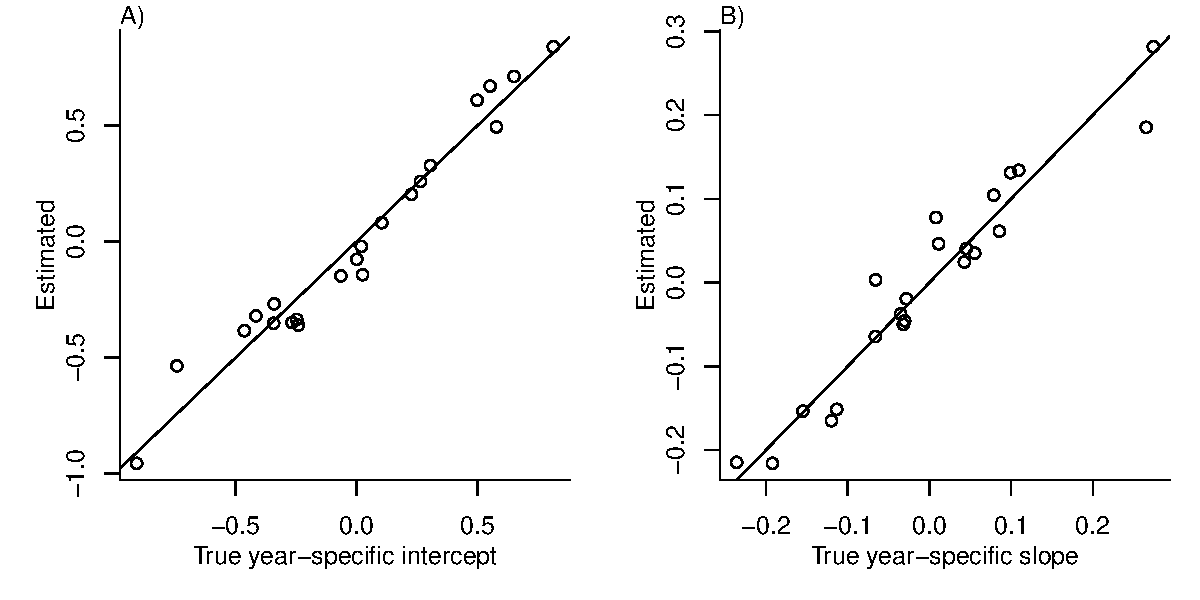
\includegraphics[width=\textwidth]{figures/SimpleShrinkage.pdf}}
		\caption{Comparison of the true random year effects with the shrinkage estimates, for one artificial data set
			generated from the fitted growth model for  \emph{Pseudoroegneria spicata}. Figure made by R script 
			\texttt{SimpleShrinkageExample.R} in our code archive.} 
		\label{fig:compareShrinkage}
	\end{figure}
	
	
	\section{Additional case studies}
	\label{sec:moreCases}
	
	\subsection{Sea fan corals, \emph{Gorgonia ventalina}}
	\label{sec:seafans}
	\cite{bruno-etal-2011} developed an IPM to understand the rise and fall of a fungal pathogen \emph{Aspergillus sydowii} in Caribbean sea fan corals \emph{G. ventalina}. 
	The model was based on repeated observations of marked corals in permanent transects at several sites near Akumal, Mexico, recording disease status (infected/uninfected) and the area of uninfected tissue. 
	The epidemic peak had passed and disease incidence was already low, so infected fans were relatively infrequent. 
	We therefore limit the analysis here to uninfected individuals.
	\citet{bruno-etal-2011} found statistically significant year and site effects, but as those explained a very small fraction of the variation in growth increments, they fitted a single growth model to data pooled across years and sites. 
	We do the same here. 
	The pooled data set consists of 358 observed size transitions. 
	The data exhibited size-dependent variance in growth (change in area, $cm^2$).  
	\cite{bruno-etal-2011} chose to stabilize the variance by cube-root transforming size, and then fitting the standard model with Gaussian growth increments. 
	Here we take a different approach, using natural log transformation of area and modeling size-dependent variance. 
	
	With initial size as the only predictor, a simple way to fit a Gaussian model with nonconstant variance is the \texttt{gam} function in \textbf{mgcv} library \citep{wood-2017} using the \texttt{gaulss} family. 
	The mean and standard deviation are both fitted as smoothing spline functions of initial size, and the \texttt{predict} function returns the fitted mean and also the inverse of the fitted standard deviations with which we can compute the scaled residuals: 
	\begin{lstlisting}
		# XH is a data frame holding the data
		# logarea.t0, .t1 denote initial and final values of log-transformed area   
		fitGAU <- gam(list(logarea.t1~s(logarea.t0),~s(logarea.t0)),
		data=XH, gamma=1.4, family=gaulss())
		fitted_all = predict(fitGAU,type="response"); 
		fitted_sd = 1/fitted_all[,2]; 
		scaledResids = residuals(fitGAU,type=''response'')/fitted_sd;  
	\end{lstlisting}
	Fig. \ref{fig:coral_diagnostics}A shows the log-transformed data and Gaussian model. 
	The mean function (solid red curve) is visually nearly linear, but the fitted spline is strongly favored over a linear model for the mean ($\Delta AIC \approx 9$). 
	The spline for standard deviation $\sigma$ versus initial size reflects the evident greater variability in growth at smaller sizes.  
	Spline regression found only very small trends in the mean or variance of scaled residuals (R script \texttt{crosssp\_diagnose\_pilot.R}; see Fig. \ref{fig:diagnose_pilot_supplement}A,B). 
	
	\begin{figure}[tbp]
		\centering
		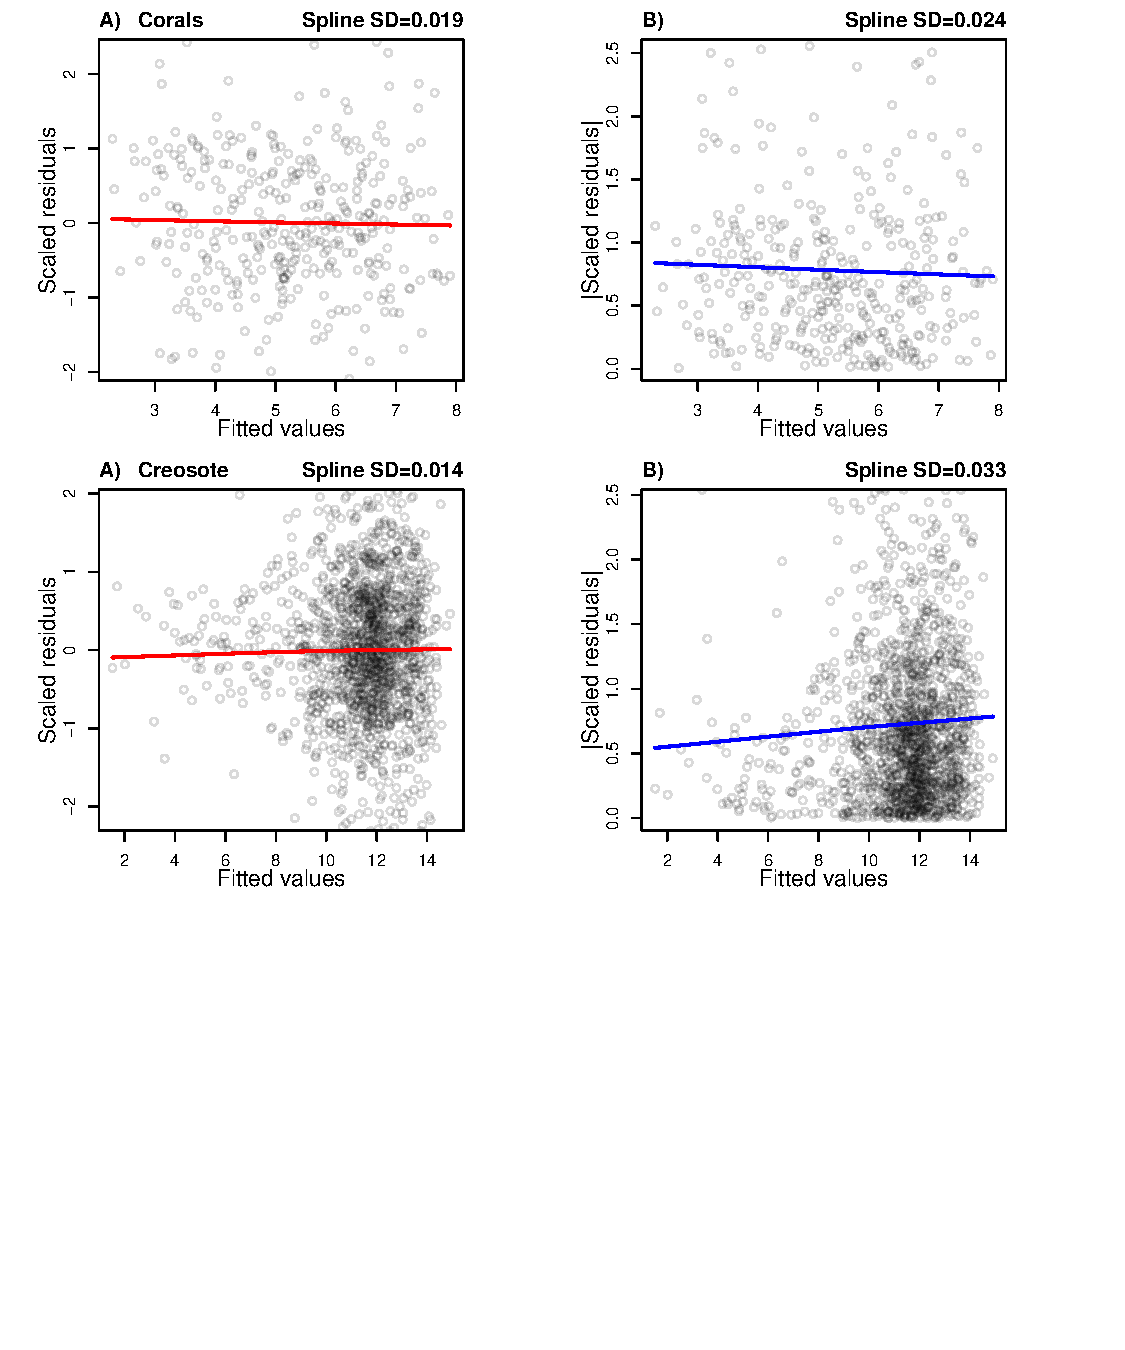
\includegraphics[width=0.95\textwidth]{figures/diagnose_pilot_supplement.pdf}
		\caption{Diagnostic plot for trends in the mean (left column) or variance (right column) of scaled residuals from a pilot Gaussian model, for the sea fan corals \textbf{A,B}, creosote bush \textbf{C,D}, and pike \textbf{E,F}. 
			In \textbf{A,C,E} the standardized residuals are plotted, and in \textbf{B,D,F} the absolute values of
			standardized residuals, as functions of fitted mean subsequent size values. The solid curves are cubic splines (R function \texttt{smooth.spline}) fitted by generalized cross-validation with a modest over-penalization of model degrees of freedom to prevent overfitting (\texttt{penalty}=1.4 as recommended by \citet{gu-2013}). The numbers appearing above each panel are the standard deviation of the values on the spline regression curve, evaluated at all of the 
			fitted values. Figure made by script \texttt{crossspp\_diagnose\_pilot.R}.}
		\label{fig:diagnose_pilot_supplement}
	\end{figure}
	
	
	\begin{figure}[tbp]
		\centering
		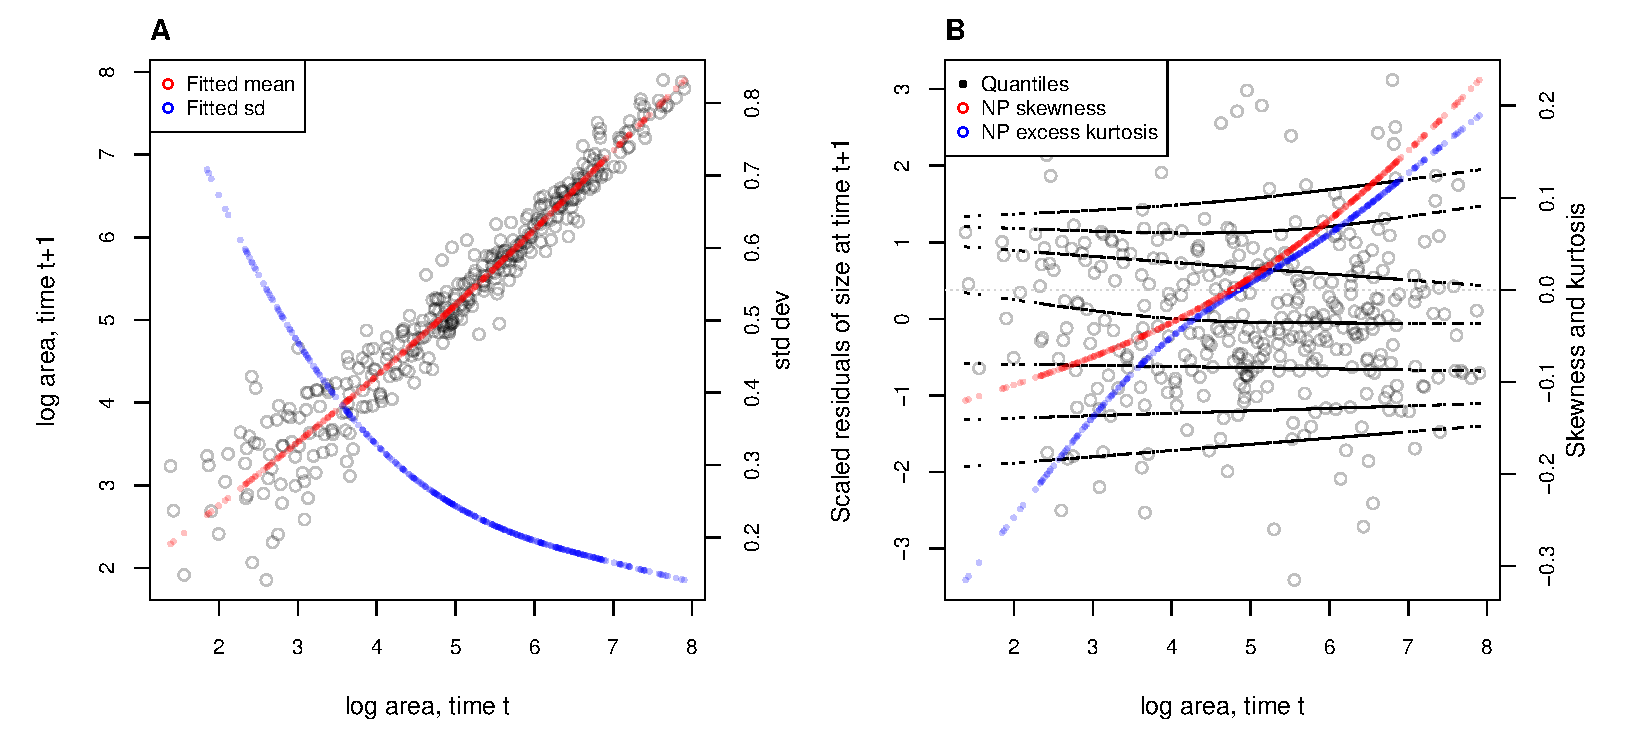
\includegraphics[width=1.0\textwidth]{figures/coral_qgam_diagnostics.pdf}
		\caption{\textbf{A}, Size transition data for sea fan corals, \emph{Gorgonia ventalina}, and fitted gam with mean (red) and standard deviation (blue) of future size conditional on current size.  \textbf{B}, Quantile regressions of scaled residuals on size and nonparametric estimates of skewness (red) and excess kurtosis (blue) derived from them. Black lines in \textbf{B} show the 5th, 10th, 25th, 50th, 75th, 90th, and 95th quantiles. Figure made by script \texttt{AkumalCorals\_qgam.R}.}
		\label{fig:coral_diagnostics}
	\end{figure} 
	
	While there are no blatant signs of trouble in the pilot Gaussian model, quantile regressions on the scaled residuals, and the NP Skewness and Kurtosis metrics derived from them (Eq. \ref{eqn:NPskew} and \ref{eqn:NPkurt}), suggest deviations from normality (Fig. \ref{fig:coral_diagnostics}B).
	Specifically, skewness switches from negative to positive across the size range, with smaller corals more prone to extreme shrinkage and larger corals more prone to extreme growth.  
	Kurtosis also changes direction over the size distribution, with thinner tails than Gaussian at small sizes and fatter tails at large sizes. 
	The fitted nonparametric moments suggest that the upper and lower tails of size transition probabilities may differ by up to 20\%, and the weight of the tails may be \>20\% greater or less than Gaussian, depending on initial size -- not overwhelming deficiencies, but not trivial either. 
	Are these deviations from normality severe enough to warrant a second, non-Gaussian iteration of growth modeling? 
	To answer that question, we simulated data from the fitted Gaussian model and examined whether key properties of the simulated data are consistent with those of the real data. 
	If the simulated data are not consistent with the real data, it is time to choose a better distribution (Fig. \ref{fig:workflow}). 
	In this case, most of 100 Gaussian model simulations are out of line with the skew at smallest and largest sizes, and excess kurtosis observed at moderately large sizes (Fig. \ref{fig:coral_fit}~CD). For at least some parts of the size distribution, a non-Gaussian model would better capture size transitions. 
	
	\begin{figure}[tbp]
		\centering
		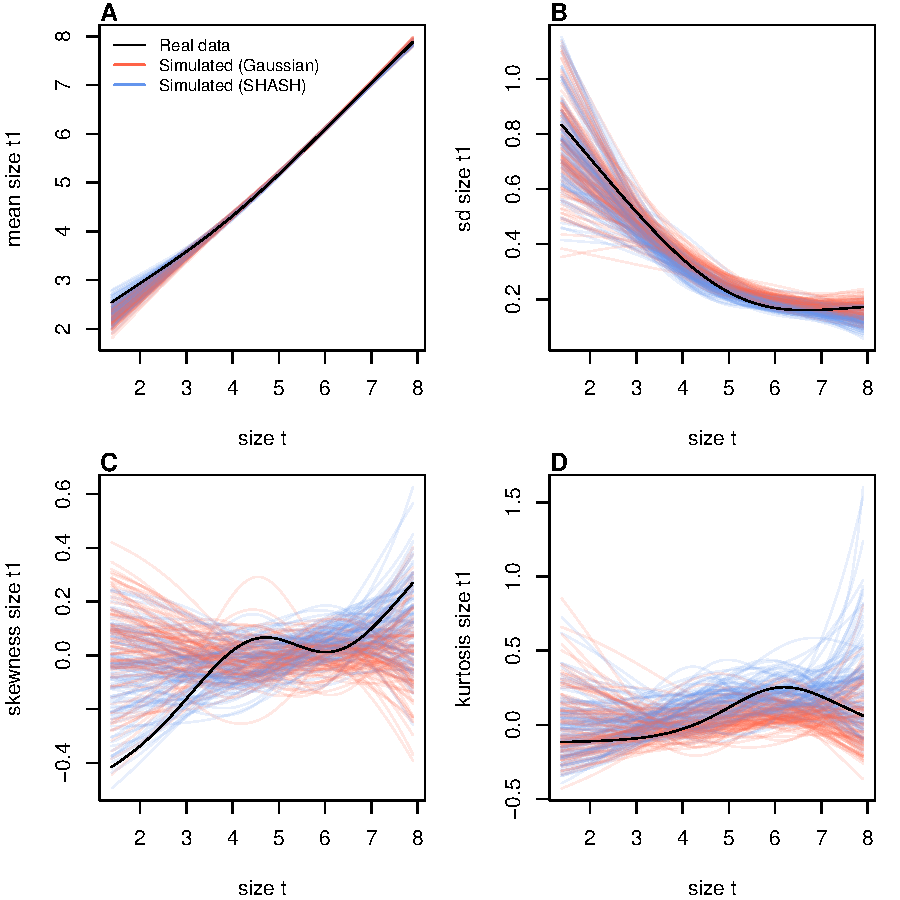
\includegraphics[width=1.0\textwidth]{figures/coral_SHASH_fit.pdf}
		\caption{Comparisons among real coral data and data simulated from Gaussian and SHASH growth models for mean, 
			standard deviation, NP skewness, and NP excess kurtosis of future size conditional on current size. Note that plotted values for the SHASH are offset by one unit to allow comparisons. 
			In the skewness and kurtosis panels, the darker solid curves show the values for the fitted growth models. 
			Figure made by script \texttt{AkumalCorals\_qgam.R}.}
		\label{fig:coral_fit}
	\end{figure} 
	
	We sought a distribution that could accommodate the observed changes in the sign of skewness and excess kurtosis. We chose the sinh-arcsinh (SHASH) distribution, a four-parameter distribution that, 
	conveniently, is included in \textbf{mgcv}'s gam() function. 
	For consistency with the Gaussian for location and scale, specification of basis functions ($k=4$) is limited to parameters for skewness and kurtosis:
	\begin{lstlisting}
		fitSHASH <- gam(list(logarea.t1 ~ s(logarea.t0), # <- location 
		~ s(logarea.t0),   # <- log-scale
		~ s(logarea.t0,k=4),   # <- skewness
		~ s(logarea.t0,k=4)), # <- log-kurtosis
		data = XH, gamma = 1.4, family = shash, optimizer = "efs")
	\end{lstlisting}
	The fitted model's mean and variance are nearly identical to the Gaussian (Fig. \ref{fig:coral_fit}AB), and the fitted trends in skewness and kurtosis are much less ``wiggly'' than the estimate from the data (Fig. \ref{fig:coral_fit}CD). 
	Nonetheless, data simulated from the SHASH model are more consistent with the real data, with more SHASH data sets matching or exceeding the largest skewness and kurtosis values observed (Fig. \ref{fig:coral_fit}CD). 
	If one cares to quantify the difference between models, the SHASH model is clearly favored by AIC ($\Delta AIC = 5.45$) despite having twice as many parameters to fit. 
	
	\begin{figure}[tbp]
		\centering
		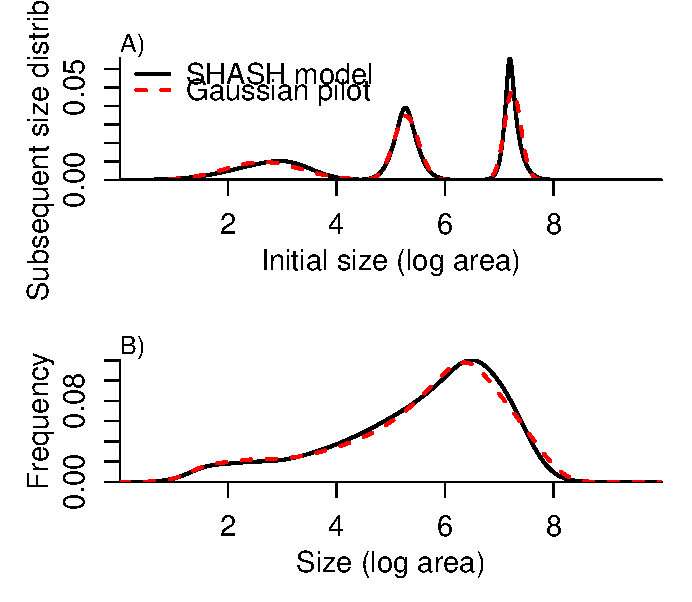
\includegraphics[width=0.95\textwidth]{figures/CoralKernelCompare_v2.pdf}
		\caption{Comparisons between the fitted \texttt{SHASH} growth model (solid black curves) and the Gaussian pilot model (dashed red curves)
			for sea fans \emph{G. ventalina}. A) Predicted frequency distributions of size in year $t+1$ for three different values of size in 
			year $t$. The leftmost pair of curves are for initial size equal to the median size of a new recruit (data from \citep{bruno-etal-2011}); 
			central pair is for the median initial size of uninfected individuals; rightmost pair are for the 95th percentile initial size for uninfected
			individuals. B) Steady-state size distributions resulting from a constant unit input of new recruits. As in \citet{bruno-etal-2011} we
			assume that larvae are very widely dispersed, so that the number of recruits arriving at any one location is independent of the local population
			abundance or structure. Size distribution of recruits was described by a kernel density estimate based on the measured sizes
			of known new recruits ($n=9$). Figure made by script \texttt{AkumalCoralsIPMs.R}.}
		\label{fig:CoralKernelCompare}
	\end{figure}   
	
	What, then, have we gained by fitting a better growth model? 
	Fig. \ref{fig:CoralKernelCompare}A compares the predicted distributions of subsequent size in the fitted model and Gaussian pilot models, for the median size of a new recruit (leftmost pair of curves), the median initial size (central curves), and the 95th percentile of initial size in the data (rightmost curves). 
	The differences are small, and most pronounced for the smallest size, where recruits are predicted to grow slightly larger under the SHASH model than the Gaussian model. 
	The direction of this difference was surprising, because the SHASH has negative skew at small sizes in the data. 
	However, the SHASH model also gives a better prediction of mean growth at small sizes than the Gaussian model. 
	At intermediate sizes the predictions are nearly identical; at large sizes the SHASH has slightly lower standard deviation, but fatter tails (excess kurtosis).  
	Fig. \ref{fig:CoralKernelCompare}B shows the predicted steady-state size distributions resulting from a constant unit input of recruits. 
	Again, the differences are very subtle. 
	Finally, the Gaussian and SHASH growth models predict very similar mean life span (17.7 and 17.9 years, respectively).
	
	In this case study we used \texttt{gam} to fit both the Gaussian and SHASH models because that obviated model selection on functions for mean, variance, and higher moments. 
	However, \texttt{gam} should be used with caution. 
	Nonparametric regression models notoriously ``wag their tails'' because the ends of the fitted curve can be pulled close to the outermost data points. 
	This is especially problematic for growth modeling, because data are typically sparse near the bounds of the size distribution. 
	To minimize the risk of overfitting we specified the number of ``knots'' (\texttt{k=4}) and used \texttt{gamma=1.4} to overweight model degrees of freedom as suggested by \citet[][sec. 3.2]{gu-2013}. 
	But it is always important to plot the fitted splines and make sure they do not wag unrealistically. 
	If they do, parametric regression may be a better choice. 
	
	\subsection{Creosotebush, \emph{Larrea tridentata}}
	\label{sec:creosotebush}
	Our next case study comes from our studies of the woody shrub creosotebush (\emph{Larrea tridentata}) at the Sevilleta Long-Term Ecological Research (LTER) site in central New Mexico, US. 
	At this site as elsewhere in the Southwest US, creosotebush is encroaching into desert grassland habitats.
	The data described here were collected along transects spanning grass-shrub ecotones to understand patterns of density dependence in creosotebush demography.
	Specifically, we asked whether fitness is maximized approaching zero density at the leading edge of the expansion front (consistent with `pulled' expansion), or whether there is a demographic advantage for shrubs at higher density due to positive feedbacks expected for ecosystem engineers (leading to `pushed' expansion). 
	Our published study \citep{drees2023demography} used a spatial integral projection model (SIPM) to predict the speed of shrub encroachment, assuming normally-distributed size transitions with non-constant variance. 
	Here we ask whether a non-Gaussian model would have been more faithful to the data, and how such an improvement would influence predictions for the speed of encroachment.
	
	Growth data come from 522 shrubs censused longitudinally over four years (2013-2017). 
	Census individuals occurred along 12 replicate transects (200 to 600 m in length) that spanned gradients of shrub density along shrub-grass ecotones. 
	Size was measured as volume of an elliptical cone based on height and width measurements; the size variable of the IPM was the natural logarithm of volume ($cm^3$). 
	For each census individual, we recorded the size and density of all conspecifics within the five-meter transect ``window'' in which it occurred, and took the sum of all sizes within the window as a weighted measure of local density. 
	The data are available in \cite{shrubdata}. 
	
	As an initial Gaussian approach, and following the approach of Drees et al. \citeyear{drees2023demography}, we first fit a generalized additive model with \textbf{mgcv} that included smooth terms for initial size and weighted density (constrained to four basis functions), plus the random effect of transect. 
	We used the \texttt{gaulss} family and, as a starting point, fit a constant standard deviation. 
	\begin{lstlisting}
		LATR_GAU <- gam(list(log_volume_t1~s(log_volume_t,k=4) + 
		s(dens_scaled,k=4) + s(unique.transect,bs="re"),~1), 
		family="gaulss", data=LATR_grow, method="ML",gamma=1.4) 
	\end{lstlisting}
	Using the fitted values from this initial model, we updated the standard deviation function to be a smooth function of fitted values, and iterated the fitting until the weights stopped changing, following the same steps as in the orchid case study. As
	with tree cholla cactus, the standard deviation function required $k=6$ basis functions to pass our graphical 
	diagnostic (Fig. \ref{fig:diagnose_pilot_supplement}C,D). The remaining small, nearly linear trend in the scale of
	standardized residuals (Fig. \ref{fig:diagnose_pilot_supplement}D) is not improved by using $k=8$ basis functions, 
	and appears to be driven by high leverage points in a region of relatively sparse data, so we did not attempt
	to further improve the pilot model. 
	
	\begin{figure}[tbp]
		\centering
		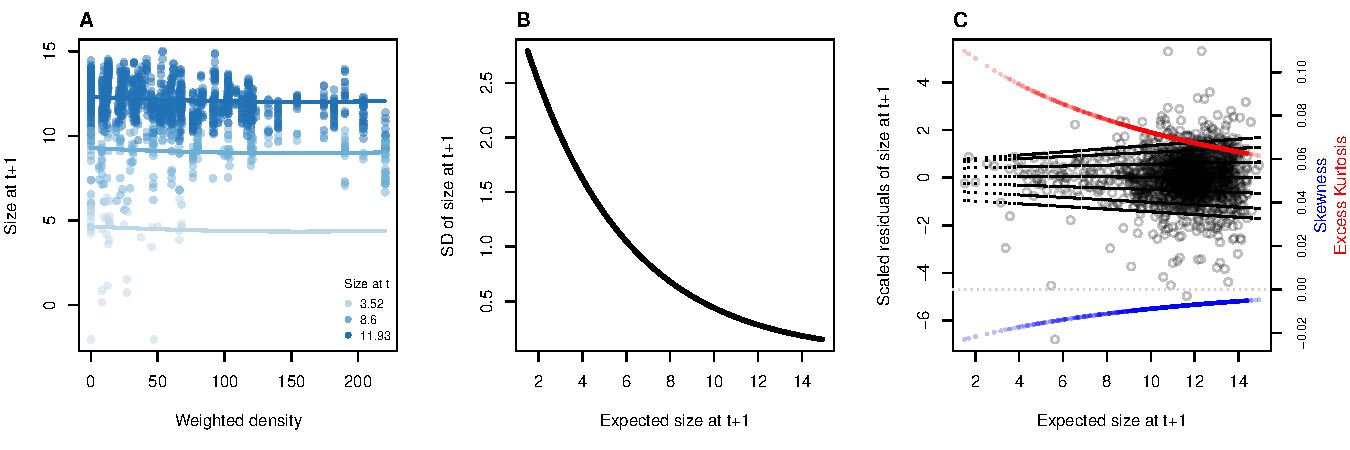
\includegraphics[width=1.0\textwidth]{figures/creosote_diagnostics.pdf}
		\caption{\textbf{A}, Creosotebush size transition data with respect to initial size (colors) and local weighted density (sum of sizes of all plants within a five-meter transect window). Size is quantified as the natural logarithm of plant volume ($cm^3$). \textbf{B}, Standard deviation of size at time $t+1$ as a function of expected size at $t+1$ (the fitted values), estimated by iterative re-weighting. \textbf{C}, Quantile regressions of scaled residuals on size and nonparametric estimates of skewness (blue) and excess kurtosis (red) derived from them. Black lines in \textbf{C} show the 5th, 10th, 25th, 50th, 75th, 90th, and 95th quantiles. All figures made by script \texttt{creosote\_growth\_modeling.R}.}
		\label{fig:creosote_diagnostics}
	\end{figure} 
	The resulting Gaussian growth model predicts strong initial size-dependence and weak and slightly nonlinear (but monotonic) negative density dependence (Fig. \ref{fig:creosote_diagnostics}A). 
	The model indicates non-constant variance, with greater dispersion at smaller sizes (Fig. \ref{fig:creosote_diagnostics}B). 
	
	
	Quantiles of the standardized residuals indicate that skew and excess kurtosis are both greater at smaller sizes (Fig. \ref{fig:creosote_diagnostics}C).
	Skewness is close to zero for larger plants (the best-sampled size range) but excess kurtosis remains positive for large plants (ca. 10\% heavier tails than Gaussian). 
	As a candidate for improvement, we turned to the Johnson's $S_{U}$ (JSU) distribution, a four-parameter, leptokurtic distribution capable of skew in either direction. 
	
	Following our suggested modeling approach, rather than re-fitting a JSU model from scratch, we parameterize a model where the residuals from the Gaussian model are fitted by a JSU distribution. 
	This is relatively easy because the \textbf{gamlss.dist} package provides a parameterization of the JSU in which the location parameter $\mu$ is the mean and scale parameter $\sigma$ is the standard deviation \citep{rigby2019distributions}. 
	We fit the ``hybrid'' model by writing a likelihood function that uses the fitted mean and standard deviation functions from Gaussian pilot model, and estimates the parameters that control skewness and kurtosis as linear functions of predicted future size.   
	The ``hybrid'' likelihood looks like this:
	\begin{lstlisting}
		JSULogLik=function(pars){
			dJSU(LATR_grow$log_volume_t1, 
			mu=LATR_grow$GAU_mean,
			sigma=LATR_grow$GAU_sd,
			nu = pars[1]+pars[2]*LATR_grow$GAU_mean,
			tau = exp(pars[3]+pars[4]*LATR_grow$GAU_mean), log=TRUE)
		}
	\end{lstlisting}
	
	The mean and standard deviation of the JSU are set to those of the best Gaussian model and parameters controlling skewness and kurtosis were fit independently, following our approach to the orchid data. 
	The hybrid JSU model performed well, generating simulated data that aligned with the real data better than the best Gaussian model, particularly in the standard deviation and kurtosis (Fig. \ref{fig:creosote_JSU}). 
	The JSU model has exactly the same mean and standard deviation of future size as the Gaussian, but Fig. \ref{fig:creosote_diagnostics} uses the quantile-based nonparametric mean and standard deviation. 
	The results show that even though the JSU was not fitted to match those, it comes closer than the Gaussian model as a result of accounting for the skew and kurtosis.
	
	\begin{figure}[tbp]
		\centering
		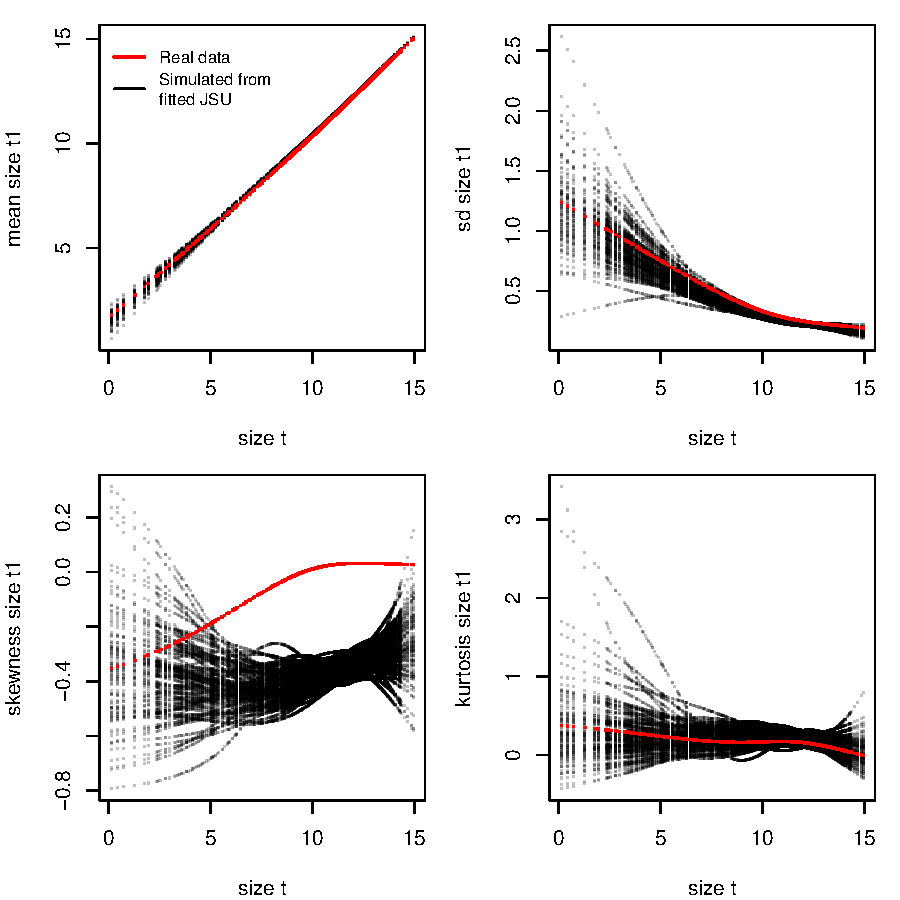
\includegraphics[width=1.0\textwidth]{figures/creosote_JSU_fit.pdf}
		\caption{Comparisons between real creosotebush data and data simulated from Gaussian and JSU growth models for nonparametric measures of mean, standard deviation, skewness, and excess kurtosis of future size conditional on current size. 
			Moments of the future size distribution are plotted with respect to initial size; their distribution is also conditional on density but initial size is by far the stronger predictor of future size, so we chose this visualization. 
			Values for the JSU model (and the corresponding ``real data'' values) are offset vertically by one unit for comparison. Figure made by script \texttt{creosote\_growth\_modeling.R}.}
		\label{fig:creosote_JSU}
	\end{figure} 
	
	The improvement of the JSU over the Gaussian growth model, while visually satisfying, had only weak influence on SIPM results. 
	The Gaussian model slightly over-estimated the low-density growth rate, but models using either Gaussian or JSU growth kernels had very similar monotonic decreases in $\lambda$ with increasing local density, and nearly identical wave velocities (Fig. \ref{fig:creosote_lambda_cstar}). 
	This species has very low mortality risk once established (mean remaining life expectancy of a median-sized shrub is 24,408 years) and its population growth and wave expansion are limited by very low seedling recruitment (\citep{drees2023demography}). 
	Weak size-dependence in survival likely explains why the improvement in growth modeling had little influence on SIPM predictions. 
	
	\begin{figure}[tbp]
		\centering
		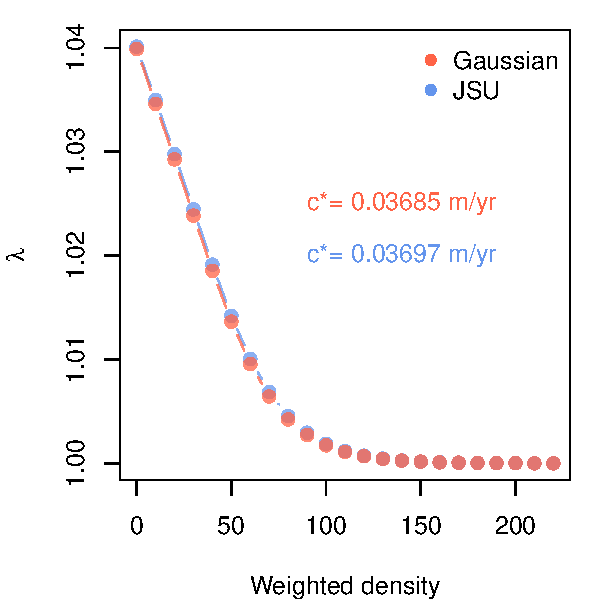
\includegraphics[width=0.5\textwidth]{figures/creosote_DD_lambda.pdf}
		\caption{Density dependence in fitness ($\lambda$) and asymptotic velocity of the creosote encroachment wave (c*) for Gaussian and JSU growth kernels. Weighted density is the sum of sizes ($log(cm^3)$) of all conspecifics within a five-meter transect ``window''. Figure made by script \texttt{creosote\_growth\_modeling\_qgam.R}.}
		\label{fig:creosote_lambda_cstar}
	\end{figure}
	
	\subsection{Case study: pike, \emph{Esox lucius}}
	\label{sec:pike}
	Our final case study comes from a long-term (51 year) study of pike (\emph{Esox lucius}) at Windemere in the English Lake District, UK. 
	Fish were gill-netted and destructively sampled to retrieve otoliths. 
	Lengths (cm) were recorded at the time of sampling and back-casted to estimate length in the preceding year. 
	There were 26501 size transitions in the data set. 
	These data are publicly available \citep{winfield2013pikegrowth}, as are data on size-specific fertility and survival \citep{winfield2013pikesurvival,winfield2013pikefecundity}, and have been analyzed in previous IPM studies \citep{vindenes2014effects,stubberud2019effects}. 
	Previous authors modeled growth using a log-normal distribution to ensure that change in length was non-negative. 
	Here, we do not attempt to reproduce the published IPMs but rather use the growth data as an additional test case of non-Gaussian growth modeling for a short-lived vertebrate. 
	
	With no additional covariates or random effects, this is a simple growth model of final size conditional on initial size. 
	We use the natural log of length. 
	Our first step was a Gaussian model of $\log(length)$ where the mean and standard deviation are smooth functions of initial size fit using the \texttt{gaulss()} family in \textbf{mgcv}. 
	We then derive the scaled residuals from the fitted mean and standard deviation:
	\begin{lstlisting}
		# pike is the data frame
		#t1 and t0 are final and inital log(length), respectively
		pike_gau<-gam(list(t1 ~ s(t0,k=5), ~s(t0,k=5)), data=pike, family=gaulss())
		pike_gau_pred<-predict(pike_gau,type="response")
		pike$fitted_mean<-pike_gau_pred,1
		pike$fitted_sd<-1/pike_gau_pred[,2]
		pike$scaledResids=residuals(pike_gau,type="response")/fitted_sd
	\end{lstlisting}
	Based on preliminary fits we found that a basis function number of $k=5$ was necessary to minimize variance trends in the standardized residuals. Even so, because of the very large sample size, our graphical diagnostics for the
	pilot mean and standard deviation functions (Fig. \ref{fig:diagnose_pilot_supplement}E,F) detected small-scale 
	deviations from constant mean and variance. Note that individual sizes in this study were recorded somewhat coarsely 
	(nearest 1cm). That accounts for the striking visual patterns in the scaled residuals, and probably also 
	accounts for the small-scale patterns in the diagnostic regression curves (Fig. \ref{fig:diagnose_pilot_supplement}E,F). 
	In order to remove the small-scale wiggles in the diagnostic splines, we would have to introduce
	small-scale wiggles in the mean and variance functions, which are unlikely to be real features of pike growth
	trajectories. So while we are not entirely satisfied with our pilot model, we see no way to improve it.
	
	The estimate growth variance strongly decreased with initial size, and size transitions were strongly positively skewed, with up to a 75\% difference in tail weight at small sizes (Fig. \ref{fig:pike_diagnostics}B). 
	Size transitions were fat-tailed at small initial sizes but were consistent with Gaussian tails at large initial sizes. 
	
	\begin{figure}[tbp]
		\centering
		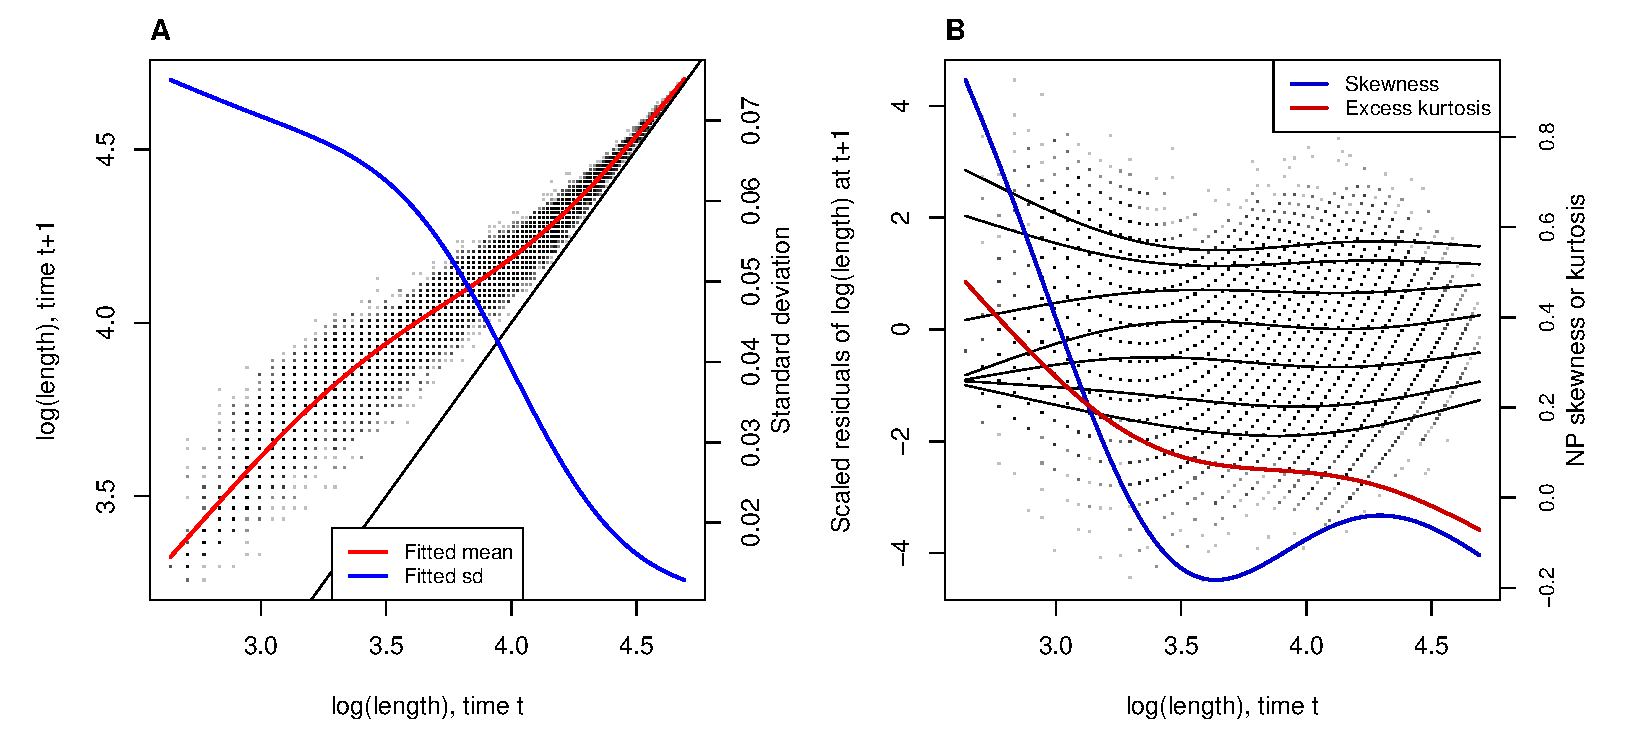
\includegraphics[width=1.0\textwidth]{figures/pike_resid_diagnostics.pdf}
		\caption{\textbf{A}, Size transition data for pike, \emph{Esox lucius}, and fitted gam with mean (red) and standard deviation (blue) of future size conditional on current size.  \textbf{B}, Quantile regressions of scaled residuals on size and nonparametric estimates of skewness (red) and excess kurtosis (blue) derived from them. Black lines in \textbf{B} show the 5th, 10th, 25th, 50th, 75th, 90th, and 95th quantiles.}
		\label{fig:pike_diagnostics}
	\end{figure} 
	
	Our improved growth model was a SHASH gam that defined all four parameters as smooth functions of initial size.
	\begin{lstlisting}
		pike_gam_shash <- gam(list(t1 ~ s(t0,k=5), # <- model for location 
		~ s(t0,k=5),   # <- model for log-scale
		~ s(t0,k=5),   # <- model for skewness
		~ s(t0,k=5)), # <- model for log-kurtosis
		data = pike, family = shash,  optimizer = "efs")
	\end{lstlisting}
	We also tried gamma regression on the change in size, to ensure strictly increasing size transitions, but found that this was not actually necessary to prevent shrinkage and did not provide as good a fit as the SHASH. 
	Data simulated from the SHASH and Gaussian models are shown in Fig. \ref{fig:pikeSims}. 
	The SHASH is an improvement over the Gaussian for most initial sizes. 
	It fails to capture kurtosis of the largest fish, but that will have little effect because the fitted mean and standard deviation imply, correctly, that those
	fish will have very small and nearly deterministic growth increments until they reach the size at which growth ceases (Figs. \ref{fig:pike_diagnostics}A, \ref{fig:pikeSims}A).  
	
	\begin{figure}[tbp]
		\centering
		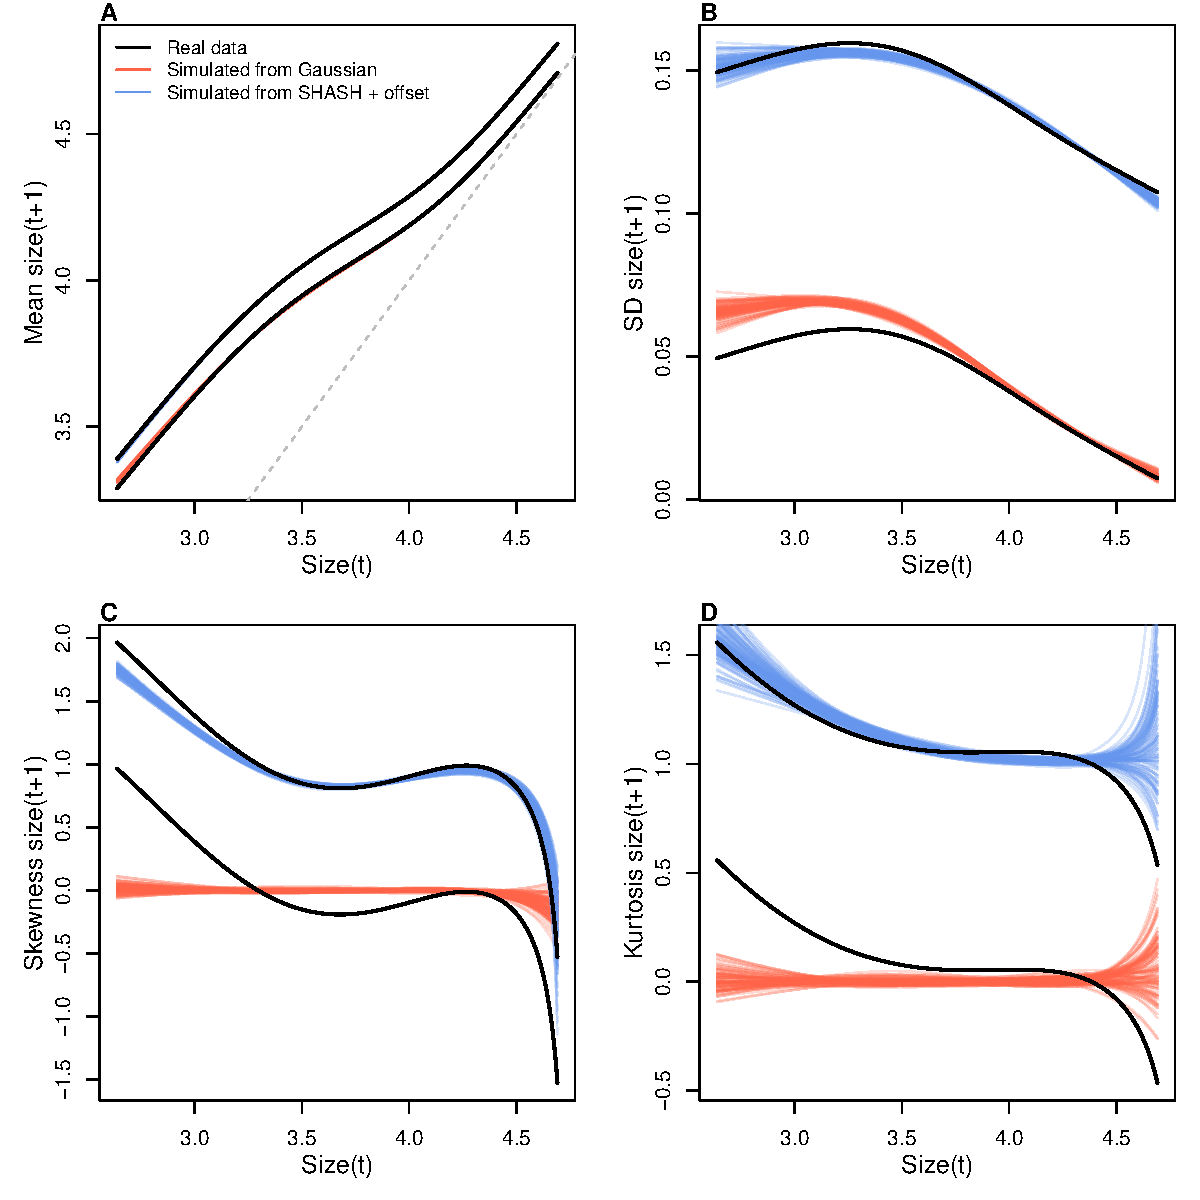
\includegraphics[width=1.0\textwidth]{figures/pike_SHASH_fit.pdf}
		\caption{Comparisons between real pike data and data simulated from Gaussian and SHASH growth models for nonparametric measures of mean, standard deviation, 
			skewness, and excess kurtosis of future size conditional on current size. 
			Moments of the future size distribution are plotted with respect to initial size. The dashed line in the top-left panel is the 1:1 line. 
			Figure made by script \texttt{PikeGrowthModeling\_qgam.R}.}
		\label{fig:pikeSims}
	\end{figure} 
	
	For the other components of the IPM, we fit GAMs for survival and egg production as smooth functions of size. 
	Parameter values for fertilization probability, fraction female (the IPM is female-dominant), and probability of survival from egg to 1-yo 
	came from \cite{stubberud2019effects}, Table 2. 
	
	Predictions from the SHASH- and Gaussian-growth IPMs (Table \ref{tab:crossspp}) are uniformly remarkably similar. 
	
	\clearpage 
	
	\section{Additional Figures}
	\label{sec:additionalFigs}
	
	\begin{figure}[h!]
		\centering
		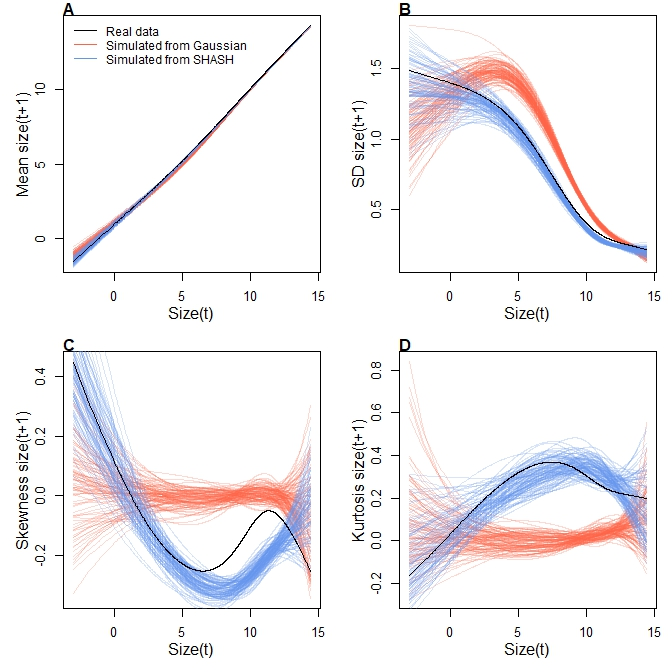
\includegraphics[width=1.0\textwidth]{figures/cactus_SHASH_fit.pdf}
		\caption{Comparisons among real cactus data and data simulated from Gaussian and SHASH growth models for mean, standard deviation, NP skewness, and NP excess kurtosis of future size conditional on current size. Figure made by script \texttt{cactus\_growth\_modeling\_qgam.R}.}
		\label{fig:cactus_fit}
	\end{figure} 
	
	\begin{figure}[h!]
		\centering
		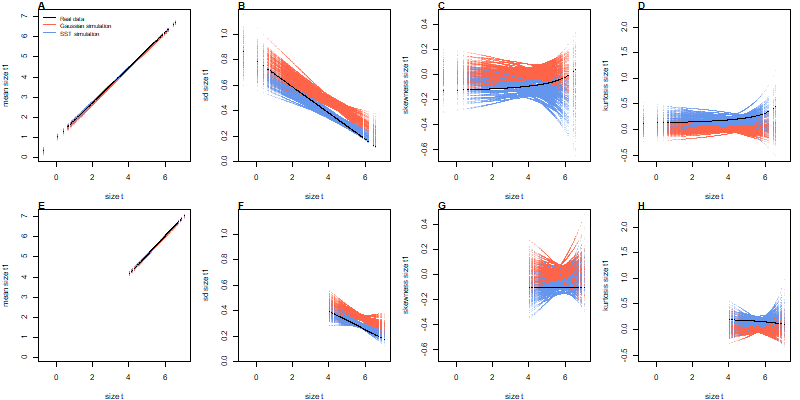
\includegraphics[width=1.0\textwidth]{figures/orchid_SST_fit.pdf}
		\caption{Comparisons between real orchid data and data simulated from Gaussian and skewed $t$ growth models for mean, standard deviation, NP skewness, and NP kurtosis of future size conditional on current size. Top row (\textbf{A}-\textbf{D}) shows plants that were vegetative at the start of the transition year and bottom row (\textbf{E}-\textbf{H}) shows plants that were flowering at the start of the transition year. Figure made by script \texttt{orchid\_growth\_modeling\_rq.R}.}
		\label{fig:orchid_SST_fit}
	\end{figure} 
	
	\clearpage
	\newpage 
	
	\begin{thebibliography}{62}
		\providecommand{\natexlab}[1]{#1}
		
		\bibitem[{Abramowitz \& Stegun(1970)}]{abram-steg}
		Abramowitz, M. \& Stegun, I.A. (1970) {Handbook of Mathematical Functions. 9th printing.}
		{D}over Publications, Inc., New York.
		
		\bibitem[{Bruno \emph{et~al.}(2011)Bruno, Ellner, Vu, Kim \&
			Harvell}]{bruno-etal-2011}
		Bruno, J.F., Ellner, S.P., Vu, I., Kim, K. \& Harvell, C.D. (2011) Impacts of
		aspergillosis on sea fan coral demography: modeling a moving target.
		\emph{Ecological Monographs} \textbf{81}, 123--139.
		
		\bibitem[{Drees \emph{et~al.}(2023)Drees, Ochocki, Collins \&
			Miller}]{drees2023demography}
		Drees, T., Ochocki, B.M., Collins, S.L. \& Miller, T.E. (2023) Demography and
		dispersal at a grass-shrub ecotone: a spatial integral projection model for
		woody plant encroachment. \emph{Ecological Monographs} p. e1574.
		
		\bibitem[{Gould \& Nichols(1998)}]{gould-nichols-1998}
		Gould, W.R. \& Nichols, J.D. (1998) Estimation of temporal variability of
		survival in animal populations. \emph{Ecology} \textbf{79}, 2531 -- 2538.
		
		\bibitem[{Jones \& Pewsey(2009)}]{jones-pewsey-2009}
		Jones, M. \& Pewsey, A. (2009) Sinh-arcsinh distributions. \emph{Biometrika}
		\textbf{96}, 761 -- 780.
		
		\bibitem[{Jones \emph{et~al.}(2011)Jones, Rosco \& Pewsey}]{jones-etal-1994}
		Jones, M.C., Rosco, J.F. \& Pewsey, A. (2011) Skewness-invariant measures of
		kurtosis. \emph{The American Statistician} \textbf{65}, 89 -- 95.
		
		\bibitem[{Link \& Nichols(1994)}]{link-nichols-1994}
		Link, W.A. \& Nichols, J.D. (1994) On the importance of sampling variance to
		investigations of temporal variation in animal population size. \emph{Oikos}
		\textbf{69}, 539 -- 544.
		
		\bibitem[{Ochocki \emph{et~al.}(2023)Ochocki, Drees \& Miller}]{shrubdata}
		Ochocki, B.M., Drees, T. \& Miller, T.E. (2023) Density-dependent demography of
		creosote bush (larrea tridentata) along grass-shrub ecotones.
		\url{https://doi.org/10.6073/pasta/ca53c16f16dcf9fb11f3ee99ea5445ac}.
		
		\bibitem[{Vindenes \emph{et~al.}(2014)Vindenes, Edeline, Ohlberger, Langangen,
			Winfield, Stenseth \& V{\o}llestad}]{vindenes2014effects}
		Vindenes, Y., Edeline, E., Ohlberger, J., Langangen, {\O}., Winfield, I.J.,
		Stenseth, N.C. \& V{\o}llestad, L.A. (2014) Effects of climate change on
		trait-based dynamics of a top predator in freshwater ecosystems. \emph{The
			American Naturalist} \textbf{183}, 243--256.
		
		\bibitem[{Winfield \emph{et~al.}(2013{\natexlab{a}})Winfield, Fletcher \&
			James}]{winfield2013pikefecundity}
		Winfield, I., Fletcher, J. \& James, J. (2013{\natexlab{a}}) Pike fecundity
		data 1963-2002. NERC Environmental Information Data Centre,
		\url{https://doi.org/10.5285/b8886915-14cb-44df-86fa-7ab718acf49a}.
		
		\bibitem[{Winfield \emph{et~al.}(2013{\natexlab{b}})Winfield, Fletcher \&
			James}]{winfield2013pikegrowth}
		Winfield, I., Fletcher, J. \& James, J. (2013{\natexlab{b}}) Pike growth data
		1944-1995. NERC Environmental Information Data Centre, \url{
			https://doi.org/10.5285/637d60d6-1571-49af-93f7-24c1279d884d}.
		
		\bibitem[{Winfield \emph{et~al.}(2013{\natexlab{c}})Winfield, Fletcher \&
			James}]{winfield2013pikesurvival}
		Winfield, I., Fletcher, J. \& James, J. (2013{\natexlab{c}}) Pike survival data
		1953-1990. NERC Environmental Information Data Centre,
		\url{https://doi.org/10.5285/813e07dd-2135-49bc-93c6-83999e442b36}.
		
	\end{thebibliography}

\end{spacing} 

\end{document}